\section{Introduction}

Many data visualizations are open to misinterpretation and misuse: patterns in raw data
can be obscured, statistical assumptions hidden, and effect sizes misrepresented
\cite{weissgerber15}. These concerns can be addressed in part through improved
statistical practices and novel plot and chart designs \cite{allen19}, but also
by making visualisations themselves more open and explorable
\cite{dragicevic19}.

One well-established technique for explorability is \emph{linked brushing}
\cite{fisherkeller75,becker87,buja91}, which shows multiple visualizations of the
same data and allows the user to interactively explore how they relate. For example,
in the geospatial domain, applications like GeoDa
\cite{anselin06} can automatically select the relevant part of one view as the
user changes the selection in a related view, say a choropleth map. Such linking
is an important navigational tool, allowing the user to switch contexts in one
view and have related views synchronise. With complex multivariate data, linking
can also be an essential sense-making aid, helping the user see relationships in
the data more readily \cite{he18}.

To support linked brushing, data visualization library needs to understand the
data transformation pipeline so that it can compute what input data correspond
to markers selected by the user and can highlight corresponding markers on another
chart. Libraries like Altair \cite{TBD} and Bokeh \cite{jolly18} support linked
brushing only for specific visual elements and with very limited data transformations
and even this is a significant coding challenge.

\begin{figure}[h]
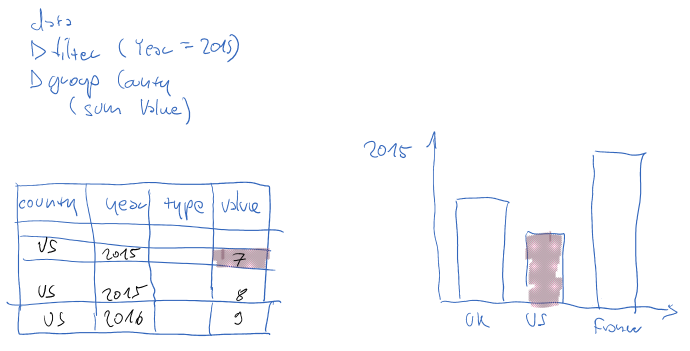
\includegraphics[scale=0.35]{image/chart-fwd}
\caption{Forward linking from code and data to visualisation}
\end{figure}

The idea of linked brushing does not have to be limited to charts. Roberts and
Wright \cite{roberts06} identify the potential utility of ``ubiquitous brushing'' for visual
elements other than plots. For example, an analyst might select a column or cell in a data
table in order to explore how particular data elements contribute to various
parts of the visualisation; equally, one might select a visual element or
attribute in order to see all the data involved in computing it.

Supporting such scenarios is beyond the capabilities of most visualization libraries today.
In this paper, we present a general framework that extends linking not only to all visual
attributes, but also to data and source code. More specifically:

\begin{itemize}
\item We motivate our work in \Secref{motivation} by example and we discuss what makes linked
  brushing challenging in the context of rich data transformation pipelines.

\item Our approach brings together work on data visualization with advances in programming
  language research. We review the problem and discuss related work in both areas
  in \Secref{background}.

\item We discuss the implementation of our system in \Secref{framework}. We evaluate our
  work in \Secref{evaluation} by referring to its formal properties and by using a case study.
\end{itemize}
